%% Graphical Abstract for the Applied Acoustics submission.
%% Legacy TikZ source retained for reference. The current submission-facing
%% image is graphical_abstract.svg -> graphical_abstract.png, because it is
%% aligned with the revised near-neutral/weak-help Conformer wording.
%% Standalone TikZ figure. Compile separately:
%%   tectonic -X compile graphical_abstract.tex
%% then submit the resulting PDF/PNG as the "Graphical Abstract" file.
%% Elsevier recommends a landscape image (about 13.3 cm x 5.3 cm).
\documentclass[border=8pt]{standalone}
\usepackage{tikz}
\usepackage{amsmath}
\usetikzlibrary{arrows.meta}
\begin{document}
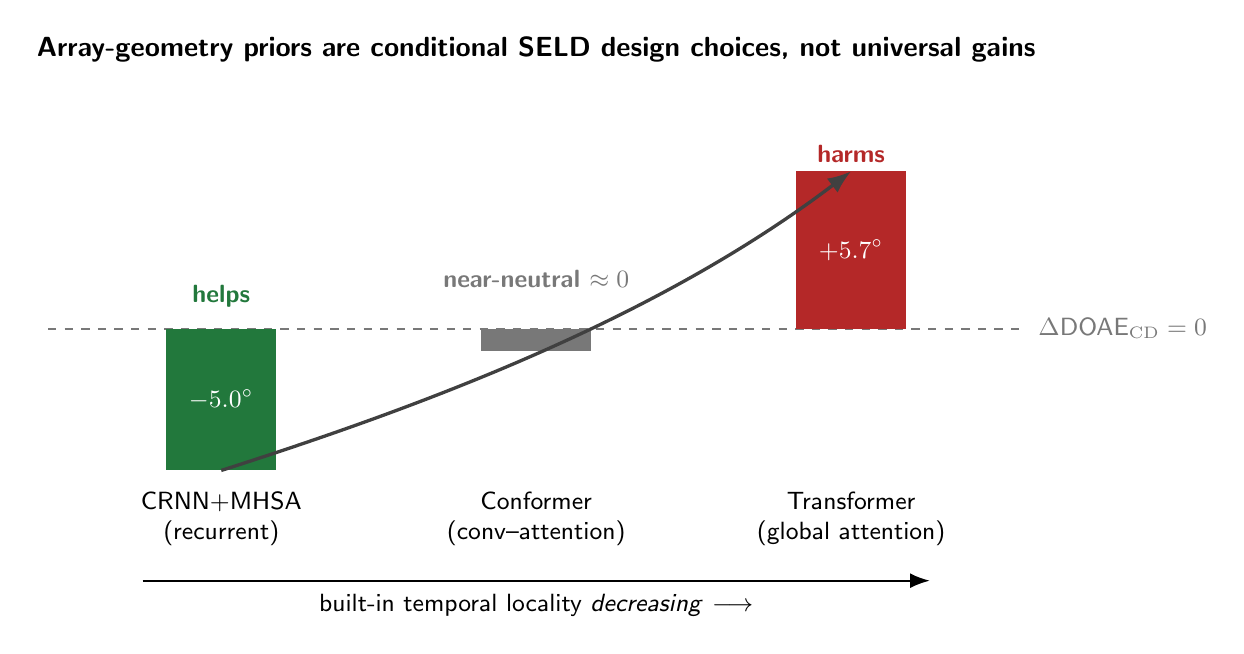
\begin{tikzpicture}[font=\sffamily]
  \definecolor{cHelp}{RGB}{34,120,60}
  \definecolor{cNeut}{RGB}{120,120,120}
  \definecolor{cHarm}{RGB}{180,40,40}

  % title
  \node[align=center,font=\sffamily\bfseries] at (6,3.55)
    {Array-geometry priors are conditional SELD design choices, not universal gains};

  % zero reference line
  \draw[cNeut,thick,dashed] (-0.2,0) -- (12.2,0);
  \node[cNeut,anchor=west,font=\sffamily\small] at (12.2,0)
    {\,$\Delta$DOAE$_{\mathrm{CD}}=0$};

  % --- Recurrent: helps (down, green) ---
  \fill[cHelp] (1.3,0) rectangle (2.7,-1.8);
  \node[white,font=\sffamily\small] at (2.0,-0.9) {$-5.0^{\circ}$};
  \node[cHelp,anchor=south,font=\sffamily\small\bfseries] at (2.0,0.15) {helps};
  \node[align=center,anchor=north,font=\sffamily\small] at (2.0,-1.95)
    {CRNN+MHSA\\(recurrent)};

  % --- Conformer: near-neutral (small, gray) ---
  \fill[cNeut] (5.3,0) rectangle (6.7,-0.28);
  \node[cNeut,anchor=south,font=\sffamily\small\bfseries] at (6.0,0.40) {near-neutral $\approx 0$};
  \node[align=center,anchor=north,font=\sffamily\small] at (6.0,-1.95)
    {Conformer\\(conv--attention)};

  % --- Transformer: harms (up, red) ---
  \fill[cHarm] (9.3,0) rectangle (10.7,2.0);
  \node[white,font=\sffamily\small] at (10.0,1.0) {$+5.7^{\circ}$};
  \node[cHarm,anchor=north,font=\sffamily\small\bfseries] at (10.0,2.45) {harms};
  \node[align=center,anchor=north,font=\sffamily\small] at (10.0,-1.95)
    {Transformer\\(global attention)};

  % trend curve through bar tops
  \draw[-{Latex[length=3mm]},very thick,black!75]
    (2.0,-1.8) .. controls (4.5,-1.0) and (7.5,0.1) .. (10.0,2.0);

  % locality axis
  \draw[-{Latex[length=2.5mm]},thick] (1.0,-3.2) -- (11.0,-3.2);
  \node[anchor=north,font=\sffamily\small] at (6.0,-3.25)
    {built-in temporal locality \emph{decreasing} $\longrightarrow$};
\end{tikzpicture}
\end{document}
